\section{Distractors Generation Algorithm}
\label{sec:distractor}
The key research topic here is to investigate a way to automatically generate suitable distractors for a certain vocabulary test. The distractors are generated in English form.
\subsection{Collecting category-related words}
To generate good category-related distractors, it is essential to gather enough words that are more related in a certain category to serve as distractors candidates. By using the approach discussed in Section 3, we crawled more than 1400 articles for seven categories, with around 200 articles in each category. The confidence factor is selected to be 10, which is suitable to classify enough words into different categories. After this step, there should be sufficient “Category-Related" words in each category.

\subsection{Generating distractors}
The category-related words obtained from the previous step will be used in this step. Out selection strategy in choosing distractors takes following parameters:
\begin{itemize}
\item News website URL
\item News sentence
\item Word to test
\item User’s knowledge level of the word
\end{itemize}
{\bf Detect news category.}
After getting the news URL, our system needs to determine the category of the news. Based on the analysis from most popular news URLs, there is a set of common identifiers that can identify the category of the news article. For example, technology news URL often contains “/tech”, “/science”, and if we find these strings in news URL, we will classify this news URL into “Technology” category. The algorithm will go through all category identifier in the list, and will return the category name the moment it finds a match. The current list of category provides reasonable accuracy for the purpose of detecting news category.

{\bf Detect Part-Of-Speech Tag.}
Given the target word and the target sentence, it is easy to run the NLTK POS tagger to get the correct POS tag of this word. This step is essential to help select distractors with similar forms, i.e. if the target word is adjective, it will be appropriate to choose three other adjectives, not verbs, as distractors.

{\bf Semantic Distance.}
Before we go to explain the next step, it is essential to introduce the semantic distance calculator we used in the server implementation. 

The perspective of semantic relatedness or its inverse, semantic distance, is a concept that indicates the likeness of two words. It is more general than the concept of similarity as stated in WordNet’s synset relation. Similar entities in WordNet are classified into same synset based on their similarity. However, dissimilar entries may also have a close semantic connection by lexical relationships  such as meronymy (car-wheel) and antonymy (hot-cold), or just by any kind of functional relationship or frequent association(pencil-paper, penguin-Antarctica) \cite{ale01}. Semantic distance calculator aims to calculate the semantic relatedness score between two words.

There are many approaches to calculate semantic relatedness score. In this application, we are using Lin Distance \cite{lin98} to calculate the semantic distance between two concepts. The detail of Lin Distance methodology is explained as follows.

Lin attempted to define a measure of semantic similarity that would be both universal and theoretically justified. There are three intuitions that he used as a basis:
\begin{itemize}
\item The similarity between arbitrary objects A and B is related to their commonality; the more commonality they share, the more similar they are;
\item The similarity between A and B is related to the differences between them; the more differences they have, the less similar they are.
\item The maximum similarity between A and B is reached when A and B are identical, no matter how much commonality they share. 
\end{itemize}

Based on the intuition above, Lin proposed his approach in measuring similarity between two concepts c1, c2 in Equation~\ref{equation:Distractor_4}:

\begin{equation}
sim(c1,c2) = \frac{2*log_p(lso(c1,c2))}{log_p(c1)+log_p(c2)}
\label{equation:Distractor_4}
\end{equation}  

where p(c) denotes the probability of encountering concept c, and lso(c1,c2) denotes the lowest common subsumer, which is the lowest node in WordNet hierarchy that is a hypernym of c1 and c2. 

The distance calculator will return a score from 0 to 1, as can be easily seen from the formula above. If the score is closer to 1, it means the two words are closer in semantic sense. This distance calculator will play an important role in the following algorithm. 

\subsubsection{Distractors Selection Algorithm}
Based on the input parameters, at this stage the server has already got the current category of the news article and the correct POS tag of the target word to test. The server is going to generate distractors based on user’s knowledge level of the target word to test.

Knowledge level is 1: This indicates that the user has just learnt this word. The algorithm will randomly select three words from current category’s word list. The reason for using randomization is to avoid the situation that similar distractors are generated every time.

Knowledge level is 2: This indicates that the user has known this word for some times. The algorithm will randomly select two words from the current category’s word list as two distractors. Then the algorithm will randomly select word from the current category’s word list and calculated the semantic distance between the selected word and the target word, once the score is above certain threshold, the selected word will be chose as the third distractor. The selection of threshold value will have a direct effect on the speed of distractors generation process. As a very high threshold value will result in more rounds of calculation in semantic distance calculator, and it will take a long time before the distractors are returned to the front end. After several rounds of analysis of each category’s words and the results returned from semantic distance calculator, the threshold value of 0.1 is selected.

Knowledge level is 3: This indicates that the user has a good understanding of the word already; the algorithm will choose distractors solely based on results returned from semantic distance calculator. Similar to the approach when knowledge level is 2, the algorithm will randomly select word from current category’s word list and calculate the semantic distance between the selected word and the target word. If the score is above certain threshold, the selected word is chosen as one of the distractors. The process is continued until the server can find three distractors. 


\subsection{Evaluation}
To evaluate the distractors selection strategy as described in this report, we chose the knowledge-based approach used by many other language learning systems, which is to utilize the WordNet data and selection distractors based on synonyms of synonyms. WordGap system uses this approach to generate vocabulary test for its android application.
\\
In our implementation of the baseline algorithm, we will choose the most frequent used word w1 from the target word’s synonym set, and select the most frequent used word w2 from word w1’s synonym set. The selection process is continued until we can find 3 distractors to form a vocabulary test. However, if the number of valid result we can get is less than 3, we will choose the word that shares the same antonym with the target word.
\\
\subsubsection{Designing Survey}
To compare the two approaches in generating distractors, we designed several survey sets to ask users to compare the plausibility of distractors. We randomly selected 50 sentences from recent news articles and choose one noun or adjective inside the sentence as the target word to test. In the survey, participants are required to answer each question and rank the plausibility of all distractors from 1 to 7. The correct answer will be ranked as 1, and the least plausible distractor will be ranked as 7. A screenshot of one sample question is shown in Figure \ref{fig:distractor_1}.
\\
\begin{figure}[ht]
   \centering
   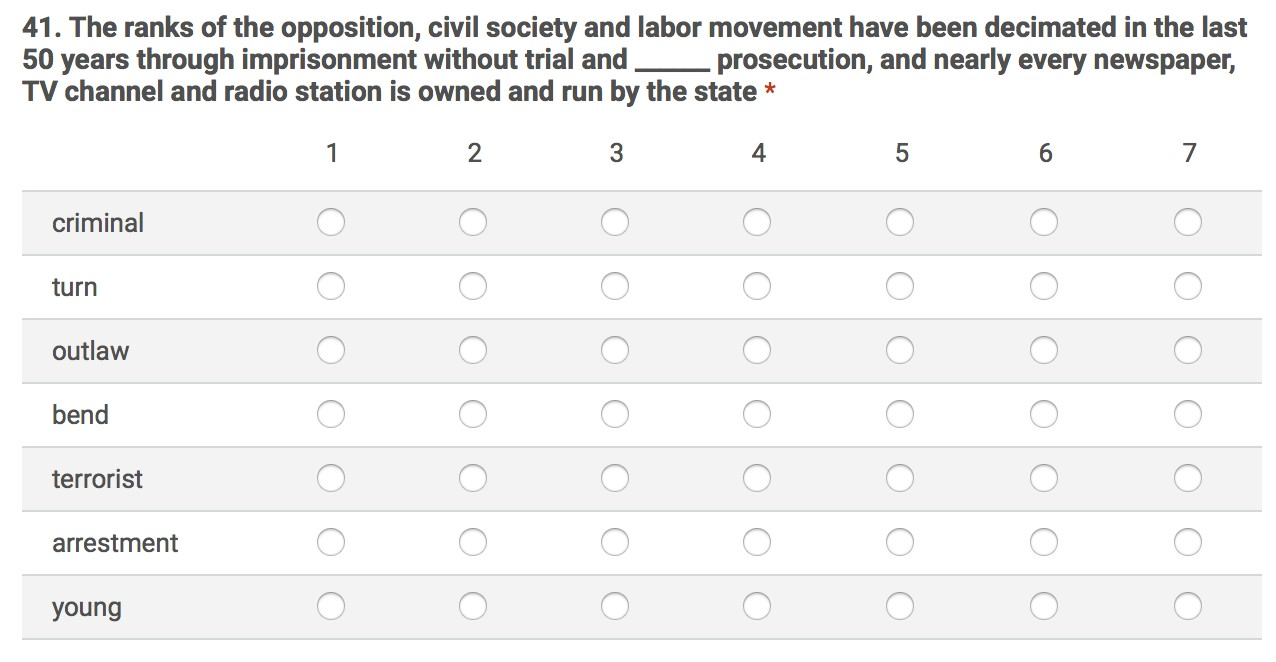
\includegraphics[width=0.45\textwidth]{distractor_1.jpg}
   \caption{A sample survey question}
   \label{fig:distractor_1}
\end{figure}
There are two evaluations to be done as follows:
1.  Compare Baseline with Knowledge Level 1 Algorithm

.  Compare Baseline with Knowledge Level 3 Algorithm
For each comparison, three distractors are generated from the baseline algorithm; three distractors are generated from the stated algorithm in this report. With the first comparison we will be able to see if the category information will help in selecting more suitable distractors. By comparing the results from the both evaluation, we will be able to see if semantic distance and category information will help improve the suitability of distractors.

\subsubsection{Results}
The evaluation contains 100 questions and is separated into 4 surveys, with each survey containing 25 questions. Each participant is free to choose one or more than one surveys. The purpose is to reduce the workload in each survey to get better responses. The surveys are sent to Year 1 students from School of Computing, National University of Singapore.  There are 15 valid responses with each participant ranking each distractor with a different weight from 1 to 7. Half of the participants are native English speakers.


Each participant’s rank will be the weight of the particular distractor in that question, i.e. if the user rank one distractor as rank “5”, the weight of this distractor in this user’s response will be 5. For each distractor of each question, the ranks of all users’ responses are summed. As the more plausible the distractor is, the higher rank it will have, thus if the sum is higher, the approach is not as plausible as the other from user’s point of view.

\begin{table}[ht]
    \caption{Comparison 1 Baseline vs. Knowledge level 1 Algorithm}
    \label{table:distractor_1}
    \begin{center}
    \begin{tabular}{| p{1.5cm} | p{2.5cm} | p{2.2cm} |}
        \hline
         & Number of winning questions & Average score\\
        \hline
        Baseline & 27 & 3.84\\
        \hline
        Level 1 Algorithm & 23 & 4.10\\
        \hline
    \end{tabular}
    \end{center}
\end{table}

\begin{table}[ht]
    \caption{Comparison 2 Baseline vs. Knowledge level 3 Algorithm}
    \label{table:distractor_2}
    \begin{center}
    \begin{tabular}{| p{1.5cm} | p{2.5cm} | p{2.2cm} |}
        \hline
         & Number of winning questions & Average score\\
        \hline
        Baseline & 21 & 4.16\\
        \hline
        Level 3 Algorithm & 29 & 3.49\\
        \hline
    \end{tabular}
    \end{center}
\end{table}

Table \ref{table:distractor_1} and Table \ref{table:distractor_2} showed the detailed result of each comparison. If for any question, the sum of weight from all participants for one approach is bigger than the other, then this approach is considered to have won this question. The “average score” is the average sum of weight from each approach for all questions. The lower the average score is, the better performance this approach has gained.

From Figure \ref{fig:distractor_1} we can see that in the first comparison, the baseline algorithm actually outscored the knowledge level 1 generation algorithm by 4 questions, with a sum of weight lower than 0.26. From Table \ref{table:distractor_1} we can see that in the second comparison, the knowledge level 3 generation algorithm surpassed the baseline algorithm by 8 questions, with the average weight of 3.49 vs 4.16. 

\subsubsection{Analysis}
In knowledge level 1 generation algorithm, there is no semantic distance calculation involved. If the target word to test has no strong category indication, for example, words like “venue”, “week”, it is possible that the knowledge level 1 algorithm will select some distractors that are not as plausible as those coming from the target word’s synonym of synonym. 

However, this problem is solved with the help of semantic distance calculator. In the knowledge level 3 generation algorithm, the distractors chosen are both semantic close and also category-related, which produced a relatively better experiment result.

Also in the baseline algorithm, it is possible that it will select words that are very rare in real life \cite{sus13}, which may also have influence in the result.
